\documentclass[runningheads]{llncs}

% ---------------------------------------------------------------
% Include basic ECCV package
% TODO REVIEW: Insert your submission number below by replacing '*****'
% TODO FINAL: Comment out the following line for the camera-ready version
\usepackage[review,year=2026,ID=*****]{eccv}
% TODO FINAL: Un-comment the following line for the camera-ready version
%\usepackage{eccv}

% ---------------------------------------------------------------
% Other packages
\usepackage{eccvabbrv}
\usepackage{graphicx}
\usepackage{booktabs}
\usepackage{amsmath}
\usepackage{multirow}
\usepackage{xcolor}
\usepackage{siunitx}
\sisetup{detect-weight=true,detect-family=true,group-separator={,}}
% axessibility.sty (PDF accessibility for math) relies on pdfTeX-only primitives
% and does not compile under XeTeX/LuaTeX. It is loaded for the pdfLaTeX
% camera-ready build (the template's default engine) and skipped otherwise, with
% no effect on layout or content. To force pdfLaTeX: ``pdflatex main''.
\usepackage{iftex}
\ifPDFTeX
  \usepackage[accsupp]{axessibility}  % Improves PDF readability for those with disabilities.
\fi

% ---------------------------------------------------------------
% Hyperref
% TODO FINAL: Comment out the following line for the camera-ready version
%\usepackage[pagebackref,breaklinks,colorlinks,citecolor=eccvblue]{hyperref}
% TODO FINAL: Un-comment the following line for the camera-ready version
\usepackage{hyperref}
\usepackage{orcidlink}

% A light convenience macro for in-draft notes. Remove before submission.
\newcommand{\todo}[1]{\textcolor{red}{[TODO: #1]}}

\begin{document}

% ---------------------------------------------------------------
\title{Single View Might Be Enough: A Task-Dependent Study of Multi-Perspective Necessity in Geosensing}

\titlerunning{Single View Might Be Enough}

% In review mode, the eccv package auto-replaces the author/institute/running
% heads with anonymous placeholders, so the real names below are only used for
% the camera-ready build. (See eccv.sty review-mode \maketitle override.)
% TODO FINAL: add ORCIDs and correct affiliations for camera-ready.
\author{Ezel Bayraktar\inst{1} \and
Alperen Demirci\inst{1} \and
Erkut Erdem\inst{1} \and
Aykut Erdem\inst{1} \and
Mukhamediyar Amanzhanov\inst{1} \and
Adam Sattout\inst{1}}
\authorrunning{E.~Bayraktar et al.}
\institute{Hacettepe University, Ankara, Turkey}

\maketitle

\begin{abstract}
Pairing overhead (satellite) and street-level imagery is widely assumed to help
vision-language models reason about cities. We test this assumption directly,
building a multi-city visual question answering benchmark of \num{40} cities in
which each location carries a satellite tile and four street-level views, with
four-way multiple-choice questions about eight urban attributes derived from
OpenStreetMap. A controlled image ablation---no image, satellite only, street
only, and both---lets us measure how much each view contributes. For these
attribute tasks the two-view condition exceeds the better single view by only
about two to three points on average, while on a built-in set of cross-view
control questions, which require both views by construction, the same model gains
$\num{17}$ to $\num{70}$ points. A paired item-level analysis shows the second
view is not merely redundant but mildly harmful: on the items it changes, it
overturns a correct answer about ten times as often as it rescues a wrong one, so
that even an oracle keeping the better single view per question beats the
two-view model. The pattern holds across a \num{9}B model we fine-tune on the
data, four off-the-shelf remote-sensing VLMs, two city splits, and three prompting
strategies including extended chain-of-thought. Multi-perspective necessity is
thus task-dependent: for urban-attribute recognition at commonly served
resolutions, one well-chosen view is competitive with two.
  \keywords{Geosensing \and Vision-language models \and Multi-view fusion}
\end{abstract}

% =====================================================================
\section{Introduction}
\label{sec:intro}

A recurring premise in geospatial machine learning is that more perspectives are
better. Overhead imagery captures layout, footprints, and connectivity; ground
imagery captures facades, surfaces, signage, and street furniture. Pairing the
two is intuitively complementary, and a growing line of work collects, aligns,
and jointly models satellite and street-level views for urban understanding.

We ask whether this expectation holds for concrete urban-attribute recognition,
and find that for the tasks we study it largely does not. We construct a
multi-city visual question answering (VQA) benchmark in which every
location is represented by a marked satellite tile and four cardinal
street-level views, and pose four-way multiple-choice questions about eight
urban attributes (land use, building height, urban density, road type, road
surface, junction type, amenity richness, and transit density) grounded in
OpenStreetMap (OSM) metadata~\cite{osm}. Crucially, the same imagery also
supports a family of \emph{cross-view} questions that are unanswerable from a
single view by construction (e.g.\ ``does this street-level photo belong to this
satellite tile?''). These cross-view tasks serve as a built-in positive control.
\Cref{fig:teaser} illustrates the setup and the headline effect on a single
location.

\begin{figure*}[t]
  \centering
  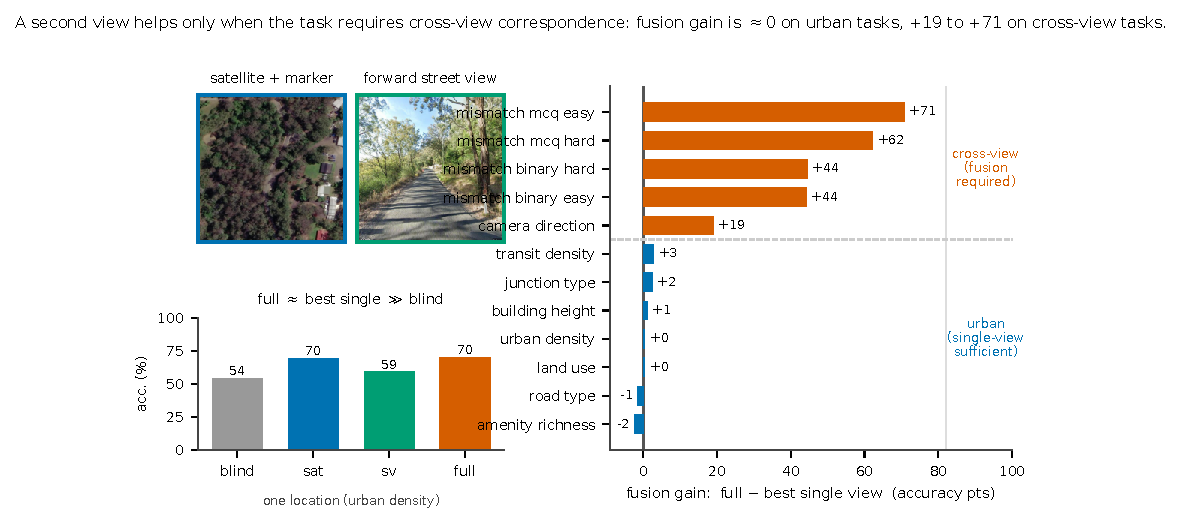
\includegraphics[width=0.82\linewidth]{figures_new/fig_teaser.pdf}
  \caption{The benchmark and the finding on one held-out location (Sydney). Each
  location pairs a marked sub-meter satellite tile with four cardinal street-level
  views; questions ask about urban attributes (here, urban density). The ablation
  (bottom right, trained Qwen3.5-9B on this task) shows the two-view condition
  (\textsf{full}) barely exceeds the better single view ($\textsf{sat}\approx
  \textsf{sv}$), while both far exceed the no-image prior (\textsf{blind}): for this
  task the second view is largely redundant. Imagery is unmodified dataset content:
  satellite tile \copyright\ Esri World Imagery; street-view panels \copyright\
  Google (Street View), shown with their original attribution.}
  \label{fig:teaser}
\end{figure*}

Our central instrument is a controlled image ablation. For each question we
evaluate a model under four input conditions---\textsf{blind} (no image),
\textsf{sat} (satellite only), \textsf{sv} (street only), and \textsf{full}
(both)---and define \emph{fusion synergy} as
$\textsf{full} - \max(\textsf{sat},\textsf{sv})$: the accuracy gained from having
both views over the better single view. Positive synergy is the signature of
genuine cross-view fusion. We complement synergy with \emph{vision contribution},
$\textsf{full} - \textsf{blind}$, which isolates how much the imagery
contributes at all over a text-only prior.

On the eight attribute
tasks, having both views improves on the better single view by only two to three
points on average---for a \num{9}B model we fine-tune on the benchmark, for four
off-the-shelf remote-sensing VLMs evaluated zero-shot, for two city splits, and
for three prompting strategies including a \num{16}k-token reasoning budget. A
paired item-level analysis (\cref{sec:itemlevel}) shows the second view is mildly
harmful rather than merely redundant: on the items where it changes the answer it
overturns a correct one about ten times as often as it rescues a wrong one
($\num{10}\%$ versus $\num{1}\%$; McNemar significant). As a result, even an oracle
that keeps the better single view per question (an upper bound, not an achievable
system) beats the two-view model by \num{8}--\num{9} points. Vision still matters
($\textsf{full}-\textsf{blind}\approx{+}\num{14}$ for the fine-tuned model): the
model reads the imagery, but one view supplies about as much usable signal as two.
On the cross-view controls the same model gains \num{17}--\num{70} points,
so the ablation detects fusion when the task requires it.

This is a \emph{task-dependent} observation about single-view-decidable attribute
recognition at commonly served satellite resolutions, not a claim that overhead
imagery is uninformative or that multi-view fusion is futile in general. We report
bootstrap confidence intervals on every synergy estimate, audit the benchmark for
text-only leakage, and characterize the items where the second view changes the
answer.

Our contributions are: (i) a multi-city satellite\,$+$\,street VQA benchmark
(\num{40} cities, eight OSM-grounded attribute tasks plus cross-view controls)
with a location-level held-out split and a four-way image ablation; (ii) the
measurement that the second view's contribution to these tasks is small and
robust across model scale, training regime, city split, and prompting strategy,
with the cross-view controls confirming the measurement is sensitive; (iii) a
paired item-level analysis showing the second view overturns about ten correct
answers for each one it rescues, so an oracle single-view router beats the
two-view model; and (iv) a reusable ablation protocol (synergy,
vision-contribution, interference asymmetry) for deciding when a second view is
warranted.

% =====================================================================
\section{Related Work}
\label{sec:related}

\subsubsection{Remote-sensing vision-language models are single-view.}
A wave of instruction-tuned VLMs target remote sensing, including
GeoChat~\cite{geochat2024}, SkySenseGPT~\cite{skysensegpt2024},
LHRS-Bot and LHRS-Bot-Nova~\cite{lhrsbot2024,lhrsbotnova2025}, EarthGPT~\cite{zhang2024earthgpt},
and the multi-sensor generalist EarthDial~\cite{earthdial2025}. These models are
overhead-only: each consumes a single aerial or satellite image, and none ingests
ground-level imagery (\cref{tab:models}). Where ``multi-modal'' appears in this
line of work it refers to multiple \emph{overhead} sensors---optical, SAR, and
infrared, as in EarthGPT---rather than to pairing satellite with street-level
views. The dominant evaluation suites follow suit: RSVQA~\cite{lobry2020rsvqa},
VRSBench~\cite{li2024vrsbench}, and GeoChat's own benchmark all pose questions
over a single overhead image. None isolates the marginal value of a second,
ground-level view, which is the question we study. Architecturally these models
build on LLaVA-style designs~\cite{llava_2023,llava15_2024} with CLIP or SigLIP
encoders~\cite{clip_2021,siglip_2023}; we use four as zero-shot baselines and
discuss their training-data provenance in \cref{sec:setup}.

\subsubsection{Multi-view urban benchmarks.}
A smaller set of benchmarks pairs overhead and ground views for urban
understanding, and two report observations that converge with ours.
UrBench~\cite{urbench2025} evaluates multimodal LLMs on coordinate-aligned street
and satellite pairs and finds little difference between multi-image and
single-image performance, attributing the gap to question comprehension rather
than fusion. The concurrent CityLens~\cite{citylens2026} benchmarks LVLMs on
socioeconomic-indicator regression from satellite and street-view and reports that
street view alone performs comparably to using both views and far above satellite
alone. That two independent studies see the same redundancy strengthens our
premise. These works do not, however, provide the per-item result at the center of
our paper: CityLens runs a three-task, single-model modality comparison on a
\emph{regression} target, and neither isolates how the second view flips
individual items or whether an oracle single-view router beats the two-view model.
We also add cross-view control tasks---absent from prior urban benchmarks---that
show the same instrument registers large fusion when fusion is required. UrbanLLaVA~\cite{urbanllava2025} trains
over satellite, street-view, OSM, and trajectory inputs but poses its
attribute-style tasks from satellite alone and reserves multi-view supervision for
matching and localization; CityCube~\cite{citycube2026} targets cross-view spatial
reasoning rather than attribute recognition.

\subsubsection{Cross-view geo-localization: where both views are necessary.}
Satellite--ground pairing is well established in cross-view geo-localization, where
the goal is to match a ground photo to an overhead
reference~\cite{durgam2024crossview,zhai2017predicting,zhu2021vigor}. There the two
views are jointly \emph{necessary}---one cannot localize the ground image without
the overhead one---and methods succeed by modeling the distinct-but-linkable layout
the views share~\cite{zhang2023geodtr}. This is the regime our cross-view controls
occupy; complementarity that is constitutive of localization is largely absent from
single-view-decidable attribute recognition.

\subsubsection{The marginal value of a second modality.}
That adding a modality need not help is known beyond geosensing. Wang
\etal~\cite{wang2020multimodal} show the best single-modal network can outperform a
naively fused one, and Liang \etal~\cite{liang2023quantifying} formalize multimodal
interaction into redundancy, uniqueness, and synergy, showing low-synergy regimes
are real; our ``fusion synergy'' is the behavioral analogue of their synergy term.
Against this, multimodal learning can provably lower achievable
risk~\cite{huang2021makes}, and several aerial$+$ground systems report recognition
gains~\cite{workman2017unified,machado2021airound}. Most directly counter to our
setting, Suel \etal~\cite{suel2021multimodal} find that fusing satellite and street
imagery improves \emph{regression} of income and deprivation; we engage this in
\cref{sec:discussion}, noting it differs in task type (regression vs.\ four-way
recognition), labels, and model (a trained CNN vs.\ our VLMs). Our finding refines
rather than contradicts the ``fusion helps'' literature by naming a regime where it
does not.

% =====================================================================
\section{The Benchmark}
\label{sec:dataset}

\subsubsection{Construction.}
The benchmark pairs overhead and street-level imagery with multiple-choice
questions about urban attributes, generated from OpenStreetMap (OSM)
metadata~\cite{osm}. Each \emph{location} is sampled within one of \num{40}
cities across \num{32} countries on six continents and is associated with (i) one
satellite tile, (ii) four street-level views at fixed bearings (forward,
backward, left, right), and (iii) OSM-derived attribute labels. Satellite imagery
is sourced per-location by geography---sub-meter aerial orthophotos: ESRI World
Imagery ($\sim$\SIrange{0.3}{0.5}{m/px} in cities) as the global default, NAIP
($\sim$\SI{0.6}{m/px}) in the US, and IGN ($\sim$\SI{0.2}{m/px}) in France, with a
coarse Sentinel-2 fallback ($\sim$\SI{10}{m/px}) reserved for locations that no
high-resolution source covers. In the benchmark every overhead tile resolves to a
sub-meter source (\num{4775} ESRI, \num{305} NAIP, \num{160} IGN; the Sentinel-2
fallback was never triggered), so the redundancy we report below is measured
against genuinely high-resolution overhead imagery rather than a coarse proxy.
The satellite tile carries a marker indicating the queried location; the marker
is part of the input condition and is held fixed across all ablation modes (we
examine its effect in \cref{sec:robustness}). The four street-level views are
retrieved from Google Street View and retain Google's original attribution;
satellite imagery is \copyright\ its respective provider (Esri, NAIP/USDA, IGN).

\subsubsection{Tasks.}
We study eight \emph{attribute} tasks---\textsf{land\_use},
\textsf{building\_height}, \textsf{urban\_density}, \textsf{road\_type},
\textsf{road\_surface}, \textsf{junction\_type}, \textsf{amenity\_richness}, and
\textsf{transit\_density}---each posed as a four-way multiple-choice question
with a single correct letter. These are the questions for which ``do we need both
views?'' is well-posed: each is, in principle, answerable from imagery of a
single location. The dataset additionally contains \emph{cross-view} tasks
(view--view matching at two difficulty levels, in binary and multiple-choice
form, and a camera-direction task) whose answer lives in the \emph{relationship}
between the two views; these are unanswerable from a single view by construction
and we use them only as a positive control (\cref{sec:control}).

\subsubsection{Splits.}
All splits operate at the location level so that no location's questions span
two splits. We hold out \num{10}\% of locations \emph{per city} as a benchmark
test set; this set is identical across training regimes and is disjoint from
training data (verified: zero question-id overlap). For training we use two
strategies that share this benchmark: a \emph{per-city} split (a further fraction
of locations per city to validation) and a \emph{seen/unseen} split (eight cities
held out entirely to validation, to probe cross-city generalization). Question
generation uses a fixed seed for option shuffling, and we keep a single question
per (location, task) pair to avoid location-level inflation. Locations with fewer
than four street-level views are discarded.

\subsubsection{Leakage audit.}
Because the questions are templated, we audit how much of each task is solvable
from text alone by evaluating every model in \textsf{blind} mode (no image) and
treat $\textsf{full}-\textsf{blind}$ as the vision-attributable signal. This audit
flagged one further attribute task (green-space presence) that a model answered at
\num{100}\% accuracy with no image, because the correct option wording was
identifiable independent of its A/B/C/D position; we \emph{exclude it entirely}
from all results, leaving the eight tasks reported here. The retained tasks show no
exploitable option-text or position regularity (\cref{sec:robustness}).

\subsubsection{Statistics.}
\Cref{tab:dataset} summarizes the benchmark. The eight-task test set comprises
\num{2932} questions over \num{421} locations across \num{40} cities; each
location supplies one satellite tile and four street-level views.

\begin{table}[t]
  \centering
  \caption{Benchmark test set (eight attribute tasks, held-out \num{10}\% of
  locations per city). Each question has four options and a single correct
  letter; image mode is a single marked satellite tile plus four street-level
  views.}
  \label{tab:dataset}
  \begin{tabular}{@{}lr@{}}
    \toprule
    Property & Value \\
    \midrule
    Cities & 40 \\
    Countries & 32 \\
    Locations (test) & 421 \\
    Questions (test) & 2932 \\
    Attribute tasks & 8 \\
    Options per question & 4 \\
    Satellite views / location & 1 \\
    Street-level views / location & 4 \\
    \midrule
    \multicolumn{2}{@{}l}{\emph{Questions per task}}\\
    \quad land\_use / urban\_density / road\_type & 421 each \\
    \quad amenity\_richness / transit\_density & 421 each \\
    \quad junction\_type & 334 \\
    \quad road\_surface & 303 \\
    \quad building\_height & 190 \\
    \bottomrule
  \end{tabular}
\end{table}

% =====================================================================
\section{Experimental Setup}
\label{sec:setup}

\subsubsection{Models.}
Our primary model is \textbf{Qwen3.5-9B} fine-tuned on the training split with
LoRA~\cite{lora_2022} (rank \num{16}, $\alpha=\num{16}$, all linear layers
including the vision tower), trained once per split and evaluated on the shared
held-out benchmark. Fine-tuning on the task distribution is the cleanest setting
for the view question, since a failure to use both views cannot then be blamed on
poor task alignment. To check that the finding is not model-specific, we also
evaluate four \emph{off-the-shelf} remote-sensing VLMs zero-shot on the overhead
half: GeoChat-7B~\cite{geochat2024}, SkySenseGPT-7B~\cite{skysensegpt2024},
LHRS-Bot-Nova~\cite{lhrsbotnova2025}, and EarthDial-4B (RGB)~\cite{earthdial2025},
all single-image overhead-only models (\cref{tab:models}).

\begin{table}[t]
  \centering
  \caption{Off-the-shelf remote-sensing VLMs evaluated zero-shot on the overhead
  (satellite-only) half of the benchmark. All four are single-image and
  \emph{overhead-only}; none ingests ground-level imagery. ``OSM data'' marks
  whether the model's training corpus is derived from OpenStreetMap (relevant to
  the contamination caveat in \cref{sec:robustness}).}
  \label{tab:models}
  \setlength{\tabcolsep}{4pt}
  \begin{tabular}{@{}lllll@{}}
    \toprule
    Model & Base LLM & Vision encoder & Input res. & OSM data \\
    \midrule
    GeoChat-7B~\cite{geochat2024}       & Vicuna-1.5-7B & CLIP ViT-L/14 & 504 & No \\
    SkySenseGPT-7B~\cite{skysensegpt2024} & Vicuna-1.5-7B & CLIP ViT-L/14 & 336 & No \\
    LHRS-Bot-Nova~\cite{lhrsbotnova2025}  & Llama-3-8B    & SigLIP-L/14   & 336 & \textbf{Yes} \\
    EarthDial-4B-RGB~\cite{earthdial2025} & Phi-3-Mini    & InternViT-300M & tiled & \textbf{Yes} \\
    \bottomrule
  \end{tabular}
\end{table}

\subsubsection{Image-ablation protocol.}
Every question is evaluated under four input conditions: \textsf{blind} (prompt
only), \textsf{sat} (the marked satellite tile only), \textsf{sv} (the four
street-level views only), and \textsf{full} (satellite tile $+$ four
street-level views). The text of the question and options is byte-identical
across conditions; only the set of supplied images changes. We decode greedily
and parse a single answer letter. For the trained model we use the same image
preprocessing as training (max edge \num{512}\,px).

\subsubsection{Metrics.}
We report per-task accuracy in each condition and two derived quantities:
\emph{fusion synergy} $\;=\textsf{full}-\max(\textsf{sat},\textsf{sv})$ and
\emph{vision contribution} $\;=\textsf{full}-\textsf{blind}$. Synergy
$>0$ indicates the second view adds accuracy a single view cannot; synergy
near zero indicates redundancy. For the trained model we attach paired bootstrap
\num{95}\% confidence intervals (\num{10000} resamples over questions) to the
pooled synergy and the item-level quantities of \cref{sec:itemlevel}.

\subsubsection{Unified harness.}
All models, trained and zero-shot, run through one harness with a shared prompt,
image rendering, and answer parsing, so the inputs are identical across models and
only the forward pass differs; runs use a single RTX\,PRO\,6000 GPU.

% =====================================================================
\section{Results}
\label{sec:results}

\subsection{The second view adds little over the better single view}
\label{sec:main}

\Cref{tab:fusion-main} reports the trained Qwen3.5-9B on the held-out benchmark,
per task, under all four conditions and both splits. First, \textsf{full} tracks
the \emph{better single view} closely: per-task fusion
synergy ranges from $-1.0$ to $+4.5$ points and averages $+\num{1.2}$/$+\num{1.3}$
points (per-city / seen-unseen) across the eight tasks. The gain is positive but
small, and street view alone (\textsf{sv}) already matches or exceeds the two-view
\textsf{full} condition on \textsf{land\_use}, \textsf{road\_type}, and
\textsf{road\_surface}. Whether this margin reflects real fusion or the model
defaulting to its stronger view is resolved at the item level
(\cref{sec:itemlevel}). Second, vision still matters: $\textsf{full}-\textsf{blind}$
is large (for example $+\num{22}$ on \textsf{transit\_density} and $+\num{32}$ on
\textsf{amenity\_richness}), so the model reads the imagery but extracts only a
single view's worth of information from it.

\begin{table}[t]
  \centering
  \caption{Trained Qwen3.5-9B on the held-out benchmark, per attribute task and
  input condition (accuracy, \%). \textbf{Syn.} $=\textsf{full}-\max(\textsf{sat},
  \textsf{sv})$ is fusion synergy. Synergy is small on every task under both
  splits; \textsf{full} stays close to the better single view.}
  \label{tab:fusion-main}
  \setlength{\tabcolsep}{4.5pt}
  \begin{tabular}{@{}lcccc@{\;}c@{\qquad}cccc@{\;}c@{}}
    \toprule
    & \multicolumn{5}{c}{\textbf{per-city split}} & \multicolumn{5}{c}{\textbf{seen/unseen split}} \\
    \cmidrule(lr){2-6}\cmidrule(lr){7-11}
    Task & blind & sat & sv & full & Syn. & blind & sat & sv & full & Syn. \\
    \midrule
    land\_use         & 68.6 & 75.5 & 75.1 & 75.3 & $-0.2$ & 63.4 & 72.0 & 72.4 & 73.9 & $+1.4$ \\
    building\_height  & 45.3 & 67.4 & 66.3 & 66.8 & $-0.5$ & 50.5 & 63.7 & 66.3 & 66.8 & $+0.5$ \\
    urban\_density    & 54.6 & 61.8 & 62.7 & 65.1 & $+2.4$ & 53.2 & 71.5 & 64.8 & 74.6 & $+3.1$ \\
    junction\_type    & 61.4 & 73.4 & 68.6 & 75.1 & $+1.8$ & 62.0 & 74.0 & 71.3 & 76.3 & $+2.4$ \\
    amenity\_richness & 26.4 & 53.4 & 56.5 & 58.7 & $+2.1$ & 25.7 & 53.0 & 55.6 & 55.6 & $+0.0$ \\
    road\_type        & 68.6 & 72.4 & 77.4 & 76.5 & $-1.0$ & 68.6 & 69.6 & 76.7 & 76.7 & $+0.0$ \\
    road\_surface     & 95.7 & 95.0 & 93.4 & 95.7 & $+0.7$ & 95.7 & 95.0 & 95.4 & 95.0 & $-0.3$ \\
    transit\_density  & 28.3 & 43.7 & 45.6 & 50.1 & $+4.5$ & 26.4 & 45.8 & 44.9 & 49.4 & $+3.6$ \\
    \midrule
    \textbf{Mean}     & 56.1 & 67.8 & 68.2 & 70.4 & $\mathbf{+1.2}$ & 55.7 & 68.1 & 68.4 & 71.1 & $\mathbf{+1.3}$ \\
    \bottomrule
  \end{tabular}
\end{table}

\subsection{The same models fuse when fusion is required (positive control)}
\label{sec:control}

Could the small attribute-task synergy reflect an insensitive measurement rather
than a real property of the tasks? \Cref{tab:control} reports the same model and
harness on the cross-view control tasks, whose answers require comparing the two
views: synergy is large, $+\num{17}$ to $+\num{70}$ points, because one view is
insufficient by construction. The same instrument reads a two-to-three-point gain on the attribute tasks and a
forty-to-seventy-point gain when the task requires both views, so the small
attribute synergy is a property of those tasks, not an insensitive test
(\cref{fig:synergy}).

\begin{table}[t]
  \centering
  \caption{Positive control: the same trained Qwen3.5-9B (per-city) on cross-view
  tasks that require both views by construction. Synergy is large and positive,
  confirming the ablation detects fusion when it is needed.}
  \label{tab:control}
  \setlength{\tabcolsep}{5pt}
  \begin{tabular}{@{}lccccc@{}}
    \toprule
    Cross-view task & blind & sat & sv & full & Syn. \\
    \midrule
    camera\_direction      & 25.2 & 24.9 & --   & 42.3 & $+17.3$ \\
    mismatch\_binary\_easy & 46.6 & 51.1 & 52.7 & 97.4 & $+44.7$ \\
    mismatch\_binary\_hard & 55.8 & 45.8 & 44.4 & 90.7 & $+44.9$ \\
    mismatch\_mcq\_easy    & 20.7 & 26.4 & 23.5 & 96.2 & $+69.8$ \\
    mismatch\_mcq\_hard    & 22.3 & 23.3 & 22.8 & 86.0 & $+62.7$ \\
    \bottomrule
  \end{tabular}
\end{table}

\begin{figure}[t]
  \centering
  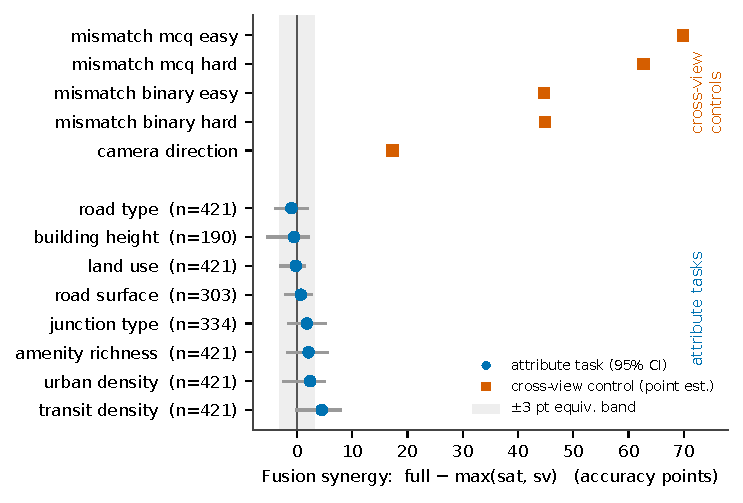
\includegraphics[width=0.74\linewidth]{figures_new/fig_synergy_control.pdf}
  \caption{Fusion synergy ($\textsf{full}-\max(\textsf{sat},\textsf{sv})$) for the
  trained Qwen3.5-9B (per-city). The eight attribute tasks (blue, with paired
  bootstrap \num{95}\% CIs) cluster near zero---most CIs span the $\pm\num{3}$-point
  equivalence band---while the cross-view control tasks (orange, point estimates)
  reach $+\num{17}$ to $+\num{70}$ points on the same axis and model. The instrument
  registers large synergy exactly when the task requires both views.}
  \label{fig:synergy}
\end{figure}

That the cross-view tasks encode cross-view information, rather than being solved
by some shortcut our VLM happens to exploit, is corroborated by an
independent, purpose-built model. A cross-view retrieval network,
Sample4Geo~\cite{deuser2023sample4geo}, transferred zero-shot and scored by cosine
similarity (a different model class and metric, not comparable to
\cref{tab:control}), reaches \num{0.65} on the binary same-place/different-place
questions---well above the \num{0.50} chance rate---confirming that the matching
tasks carry genuine cross-view signal; the attribute tasks offer no comparable
signal to recover.

\subsection{The finding holds zero-shot across off-the-shelf RS-VLMs}
\label{sec:zeroshot}

To rule out that the redundancy is an artifact of our particular model, we
evaluate four off-the-shelf remote-sensing VLMs zero-shot on the overhead
(satellite-only) half of the benchmark (\cref{tab:zeroshot}). None was trained on
our task, our four-way MCQ format, or our marker overlay. They span CLIP- and
SigLIP-based encoders, three LLM families, and single-crop versus tiled
preprocessing. The trained Qwen3.5-9B in its satellite-only mode is the
like-for-like single-overhead-view comparison; it outperforms the best zero-shot
model (EarthDial, $\num{39.9}\%$) by $+\num{26.7}$ points overall, as expected
for a model fine-tuned on the distribution. The four zero-shot models are
satellite-only and therefore inform the single-view baseline and the
contamination discussion (\cref{sec:robustness}), not the synergy claim itself,
which is a within-model comparison.

\begin{table}[t]
  \centering
  \caption{Off-the-shelf RS-VLMs, zero-shot, single marked satellite tile,
  per-task accuracy (\%) over the eight-task benchmark ($n=\num{2932}$). Last
  column: our trained Qwen3.5-9B in satellite-only mode (per-city), the
  like-for-like single-overhead-view reference. LHRS-Bot-Nova and EarthDial are
  trained on OSM-derived text and their scores should be read as an
  \emph{upper bound} on visual skill (see \cref{sec:robustness}).}
  \label{tab:zeroshot}
  \setlength{\tabcolsep}{4pt}
  \begin{tabular}{@{}lccccc@{}}
    \toprule
    Task & GeoChat & SkySenseGPT & LHRS-Nova & EarthDial & \textit{Ours (sat)} \\
    \midrule
    land\_use         & 48.7 & 53.4 & 46.3 & 47.5 & \textit{75.5} \\
    building\_height  & 30.5 & 34.7 & 28.9 & 32.6 & \textit{67.4} \\
    urban\_density    & 13.5 & 14.5 & 17.8 & 30.4 & \textit{61.8} \\
    road\_type        & 10.7 & 18.1 & 26.1 & 46.1 & \textit{72.4} \\
    road\_surface     & 75.6 & 80.2 & 58.7 & 58.4 & \textit{95.0} \\
    junction\_type    &  8.4 & 30.8 & 35.3 & 52.7 & \textit{73.4} \\
    amenity\_richness & 13.5 & 12.6 & 17.8 & 25.4 & \textit{53.4} \\
    transit\_density  & 21.4 & 26.1 & 34.2 & 29.7 & \textit{43.7} \\
    \midrule
    \textbf{Overall}  & 26.2 & 32.0 & 32.4 & \textbf{39.9} & \textit{\textbf{66.6}} \\
    \bottomrule
  \end{tabular}
\end{table}

\subsection{Stronger reasoning improves single-view reading, not fusion}
\label{sec:strategies}

If the two views \emph{were} complementary but the model simply failed to
combine them, a stronger reasoning procedure should surface the latent signal. It
does not. \Cref{tab:strategies} reports three strategies---plain decoding, a
\num{16}k-token explicit-thinking budget, and a four-turn
\emph{observe$\rightarrow$reason$\rightarrow$self-check$\rightarrow$commit}
conversation---on the eight attribute tasks, here using an AWQ-quantized
Qwen3.5-9B so the long-context reasoning runs fit a single GPU. More deliberation
raises accuracy modestly---the model gets better at each task in every
view---but synergy stays \emph{negative} throughout, and indeed \textsf{sv} alone
is the single strongest condition under every strategy. The extra reasoning
accrues to the single-view conditions just as much as to \textsf{full}, so what
improves is the model's reading of one view, not its ability to combine two. This
mirrors the item-level finding of \cref{sec:itemlevel}: the obstacle is
adjudicating between redundant views, which more thinking does not remove.

\begin{table}[t]
  \centering
  \caption{Prompting strategies on the eight attribute tasks (Qwen3.5-9B-AWQ,
  $n=\num{2932}$, per-task means). \textbf{Syn.} $=\textsf{full}-\max(\textsf{sat},
  \textsf{sv})$; \textbf{Vis.} $=\textsf{full}-\textsf{blind}$. Reasoning improves
  accuracy but not synergy---the second view remains redundant, and street-view
  alone (\textsf{sv}) is the single strongest condition in every strategy.}
  \label{tab:strategies}
  \setlength{\tabcolsep}{6pt}
  \begin{tabular}{@{}lccccrr@{}}
    \toprule
    Strategy & blind & sat & sv & full & Syn. & Vis. \\
    \midrule
    plain                 & 41.0 & 46.5 & 54.2 & 51.7 & $-2.8$ & $+10.8$ \\
    think-16k             & 41.4 & 48.2 & 54.0 & 52.5 & $-2.0$ & $+11.2$ \\
    multistep (4-turn)    & 43.4 & 50.3 & 55.0 & 53.2 & $-2.1$ & $+9.8$ \\
    \bottomrule
  \end{tabular}
\end{table}

\subsection{Item-level analysis: the second view interferes more than it helps}
\label{sec:itemlevel}

A small positive average could still hide genuine fusion on a subset of items. We
join the predictions of all four conditions at the item level---every benchmark
question carries a stable identifier shared across conditions---and analyze the
\num{2932} fully paired eight-task items directly.

\subsubsection{The second view overturns far more correct answers than it rescues.}
Comparing \textsf{full} against the better single view on each item is label-free
and direct (\cref{tab:oracle}). First, genuine fusion is rare: \textsf{full} is correct while
\emph{both} single views are wrong on only \num{26} items ($\num{0.9}\%$, per-city)
and \num{35} items ($\num{1.2}\%$, seen/unseen). Second, interference is common:
\textsf{full} is wrong while at least one single view was right on \num{298} items
($\num{10.2}\%$) and \num{267} items ($\num{9.1}\%$). The second view therefore
overturns a correct answer roughly ten times as often as it rescues a wrong one. A
McNemar test on the paired \textsf{full}-versus-single outcomes confirms the
imbalance is not noise ($p<\num{e-3}$ for \textsf{full} vs.\ either single view on
both splits; e.g.\ \num{219} vs.\ \num{133} discordant items for \textsf{full} vs.\
\textsf{sat}, per-city, $p=\num{5e-6}$). When the two views disagree, the model
does not reliably keep the correct one; the extra view is, on net, a distractor.

\subsubsection{An oracle single-view router would beat the two-view model.}
The same asymmetry can be stated as an upper bound. Consider an \emph{oracle} that,
per item, keeps the better of the two single-view answers---a router, not a
fusion model, and not an achievable system, since selecting the right view uses the
gold label. This upper bound on single-view \emph{routing} exceeds \textsf{full}
by $\num{9.3}$ points (per-city) and $\num{7.9}$ points (seen/unseen), with paired bootstrap \num{95}\% intervals
that exclude zero ($[\num{-10.4},\num{-8.2}]$ and $[\num{-9.1},\num{-6.8}]$,
\num{10000} resamples; \cref{tab:oracle,fig:oracle}).

\subsubsection{Aggregate synergy is small and positive---not zero.}
The average gain is not zero. \Cref{tab:oracle} reports the
pooled fusion synergy with its bootstrap CI: $+\num{2.2}$ $[\num{0.9},\num{3.3}]$
(per-city) and $+\num{2.8}$ $[\num{1.5},\num{3.7}]$ (seen/unseen); both intervals
sit above zero. (These item-weighted pooled values slightly exceed the
$+\num{1.2}$/$+\num{1.3}$ unweighted task means of \cref{tab:fusion-main} because
the larger tasks carry the larger synergies.) An equivalence test (TOST,
\cite{lakens2018tost}) against a
$\pm\num{3}$-point margin does \emph{not} declare the synergy negligible---it is a
real, small, positive effect. Our claim is correspondingly bounded: the second view
adds a couple of points on average, more than an order of magnitude below the
$+\num{17}$ to $+\num{70}$ points it adds on the cross-view controls
(\cref{tab:control}), while breaking roughly one in ten items it touches. Whether a
$\sim$\num{2}-point average gain at that cost warrants serving a second imagery
modality is the practical question we take up in \cref{sec:discussion}.

\begin{table}[t]
  \centering
  \caption{Item-level analysis on the \num{2932} paired eight-task questions.
  \textbf{Fusion-win} = items \textsf{full} answers correctly while \emph{both}
  single views fail; \textbf{Interfere} = items \textsf{full} fails while at least
  one single view succeeded. \textbf{synergy} $=\textsf{full}-\max(\textsf{sat},
  \textsf{sv})$ and \textbf{full$-$oracle} (oracle keeps the better single-view
  answer per item; an upper bound on single-view routing, not an achievable system)
  carry paired bootstrap \num{95}\% CIs (\num{10000} resamples). The second view
  rescues few items and breaks many more.}
  \label{tab:oracle}
  \setlength{\tabcolsep}{4.5pt}
  \begin{tabular}{@{}lcccccc@{}}
    \toprule
    Split & full & synergy & oracle & full$-$oracle & Fusion-win & Interfere \\
    \midrule
    per-city    & 69.5 & $+2.2$ \footnotesize$[0.9,3.3]$ & 78.8 & $-9.3$ \footnotesize$[-10.4,-8.2]$ & 0.9\% & 10.2\% \\
    seen/unseen & 70.3 & $+2.8$ \footnotesize$[1.5,3.7]$ & 78.2 & $-7.9$ \footnotesize$[-9.1,-6.8]$ & 1.2\% & 9.1\% \\
    \bottomrule
  \end{tabular}
\end{table}

\begin{figure}[t]
  \centering
  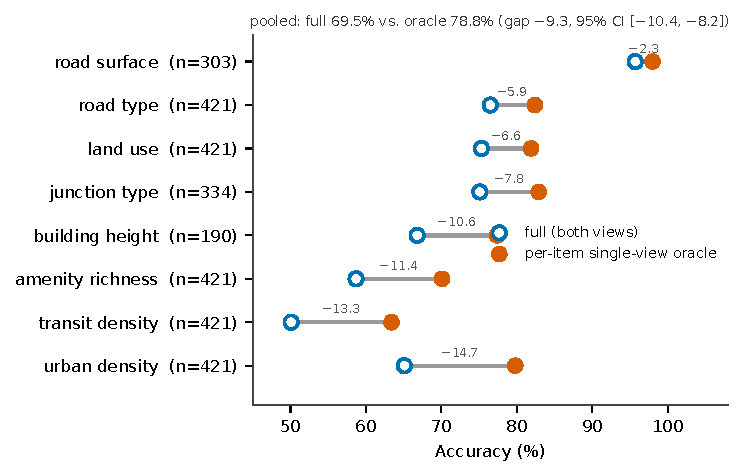
\includegraphics[width=0.72\linewidth]{figures_new/fig_oracle_dumbbell.pdf}
  \caption{Per task, the two-view \textsf{full} condition (open circles) versus a
  per-item single-view oracle that keeps the better single-view answer for each
  question (filled circles; an upper bound on single-view routing, not an
  achievable system). The oracle leads on every task. Trained Qwen3.5-9B,
  per-city.}
  \label{fig:oracle}
\end{figure}

% =====================================================================
\section{Robustness and Confounds}
\label{sec:robustness}

\subsubsection{Option text and position.}
Because the questions are templated, we check that the answer cannot be read off
the options. The correct letter is close to uniform across the eight retained
tasks (A/B/C/D $=$ \num{743}/\num{766}/\num{703}/\num{720}; $\chi^2=\num{3.08}$,
$p=\num{0.38}$ against uniform), and the correct option is not systematically the
longest---its mean length (\num{24.0} characters) is slightly below that of the
distractors (\num{25.0}), and it is the single longest option on only
$\num{19.8}\%$ of items, below the $\num{25}\%$ chance rate. The \textsf{blind}
accuracy we report per task (\cref{sec:main}) is the empirical ceiling on
everything guessable without images and subsumes these effects.

\subsubsection{Text-only leakage and degenerate tasks.}
We exclude the one task that was fully text-solvable (\cref{sec:dataset}). One
retained task, road surface, is near ceiling and almost text-solvable
($\textsf{blind}=\textsf{full}=\num{95.7}$, vision contribution $\approx 0$), so
its small synergy reflects that nothing in the image matters, not redundancy
between views. Restricting the headline finding to the seven tasks with a
meaningful vision contribution ($\textsf{full}-\textsf{blind}>\num{5}$ points)
leaves the conclusion unchanged: mean synergy is $+\num{1.5}$ points
($n=\num{2629}$). We therefore rank and interpret tasks by vision contribution
rather than raw accuracy throughout.

\subsubsection{OSM provenance.}
Our labels are OSM-derived. Two of the four zero-shot models---LHRS-Bot-Nova and
EarthDial---are trained on OSM-derived text (LHRS-Align captions OSM tags across
\num{9259} cities; EarthDial's pretraining QA is built from OSM-labeled imagery),
so their scores may reflect shared OSM priors, and we treat them as an upper bound
on visual skill; GeoChat and SkySenseGPT do not share this provenance. The synergy
result, however, is a \emph{within-model difference} (\textsf{full} vs.\ the
better single view), so any view-independent OSM prior cancels in the difference
and cannot produce the effect.

\subsubsection{Satellite resolution.}
The redundancy is measured against high-resolution overhead imagery, not a coarse
proxy: every benchmark tile resolves to a sub-meter source (ESRI
$\sim$\SIrange{0.3}{0.5}{m/px}, NAIP $\sim$\SI{0.6}{m/px}, IGN
$\sim$\SI{0.2}{m/px}); the Sentinel-2 fallback ($\sim$\SI{10}{m/px}) is never
triggered. For tasks that are structurally ground-level (road surface,
signage-driven amenities) no overhead resolution recovers the cue. We cannot rule
out that still higher ground sampling distance would help the few tasks where
overhead geometry is plausibly resolution-limited (building height, urban
density); we flag this as the main open question in \cref{sec:limitations}.

\subsubsection{Image count and attention.}
The street-view condition supplies four images and the satellite condition one, so
part of street view's edge could be image count rather than viewpoint. Three points
bound this concern. First, our headline result does not require
$\textsf{sv}>\textsf{sat}$: it is stated against the \emph{better} single view,
whichever that is, and the interference asymmetry holds regardless. Second, an
attention check argues against a pure token-count effect---on a separate
attention-instrumented model, the raw cross-modal attention at the answer token
favors street view ($\num{6.3}\%$ vs.\ $\num{2.0}\%$), but \emph{per image} the
satellite tile draws \emph{more} attention than any single street view
($\num{24.3}\%$ vs.\ $\num{18.9}\%$), so the satellite tile is read at least as much
as one street view (attention is reported only as corroboration; its limits as
explanation are well known~\cite{jain2019attention,wiegreffe2019attention}).
Third, our recommendation is to serve the cheaper single view, so street-view
richness is part of why one view suffices. We did not, however, equalize image
count directly by comparing a single street-level angle to the four-view grid, and
flag that as a limitation (\cref{sec:limitations}).

% =====================================================================
\section{Discussion}
\label{sec:discussion}

Our reading is that complementarity is a property of the task rather than of
imagery in general. An attribute question, such as the local land use, building
height, or road surface, can be answered from one location's imagery, and the two
views then encode much the same answer-relevant content, so the model reads it off
whichever view is more convenient. A cross-view question (whether a street photo
belongs to a given tile, or which way a camera points) instead depends on the
relationship between the views, where our models do use the second view. The eight
attribute tasks fall in the first regime, the cross-view tasks in the second.

This has a practical consequence. Street-level and high-resolution satellite
imagery differ sharply in cost, coverage, and licensing, yet for these attribute
families the second view adds only two to three points and naively degrades about
one item in ten. A deployment can serve a single view, the cheaper or
better-covered one, at little accuracy cost; and when both are available, the
evidence favors \emph{routing} each question to one view over feeding the model
both. The synergy, vision-contribution, and interference measures we use form a
reusable instrument for making that call before committing to dual-view
collection.

\subsection{Limitations and scope}
\label{sec:limitations}

The claim concerns eight urban-attribute tasks in four-way MCQ form at commonly
served satellite resolutions; it is not a claim that overhead imagery is
uninformative or that fusion fails in general, as the cross-view controls show
large synergy on the same models. Four caveats bound it further: we did not
equalize image count between the single-view conditions (\cref{sec:robustness});
our two splits are two training regimes on one shared held-out test set, of which
the held-out-cities split is the true generalization check; higher ground sampling
distance might help the few overhead-geometry-limited tasks (building height, urban
density); and an open-ended or regression formulation could surface complementary
signal an MCQ cannot express.

% =====================================================================
\section{Conclusion}
\label{sec:conclusion}

We measured, rather than assumed, the value of a second perspective for urban
attribute recognition. Across model scale, training regime, city split, and
prompting strategy the second view adds only a few points over the better single
view and overturns a correct answer about ten times as often as it rescues a wrong
one, while the same models gain \num{17}--\num{70} points on cross-view tasks that
require both views. Multi-perspective necessity is thus task-dependent; for these
urban-attribute tasks, a single well-chosen view might be enough.

% ---------------------------------------------------------------
% TODO FINAL: remove for camera-ready; required for review.
\clearpage

%\section*{Acknowledgements}
% TODO FINAL: add acknowledgements (no section number).

\bibliographystyle{splncs04}
\bibliography{eollm,main}
\end{document}
